\begin{frame}{\insertsubsection}

  CVE-2017-5753: обход проверки границ

  \begin{figure}[h]
    
\includegraphics[height = .7\textheight]{spectre_logo}
    % \caption{Spectre}
  \end{figure}

  \note{


  }
\end{frame}

\subsubsection{Необходимые условия}
\begin{frame}{\insertsubsubsection}
  \begin{itemize}
  \item Спекулятивное выполнение кода
  \item Присутствие необходимых гаджетов в коде
  \item Обход других систем защиты в коде
  \item Точные счётчики времени
  \item и др.
  \end{itemize}

  \note{

    \begin{itemize}
    \item Ожидаемое поведение при спекулятивном выполнении кода.
    \item Составляется особая ROP цепочка для эксплуатации, которая
      \textbf{помещается в спекулятивное окно}.
    \item Обход \textbf{ASLR} другими атаками.
    \item Для реализации атаки на кэш.
    \end{itemize}

  }
\end{frame}

% \subsubsection{Спекулятивное выполнение}
% \begin{frame}{\insertsubsubsection}

%   \begin{itemize}
%   \item CPU пытается предугадать будущие переходы
%     \begin{itemize}
%     \item ... учась на произошедших
%     \end{itemize}
%   \item происходит спекулятивное выполнение инструкций выбранного перехода
%   \item если переход угадан верно
%     \begin{itemize}
%     \item ... быстрое выполнение
%     \end{itemize}
%   \item если переход угадан неверно
%     \begin{itemize}
%     \item ... отброс результата спекулятивного выполнения
%     \end{itemize}
%   \end{itemize}

%   \note{

%     Вскользь уже была упомянута тема с предугадыванием переходов.

%     Какие же \textbf{побочные эффекты} могут нас ожидать при такой архитектуре?

%   }
% \end{frame}

% \subsubsection{Побочные эффекты}
% \begin{frame}{\insertsubsubsection}

%   \begin{figure}[h]
%     \begin{tikzpicture}[
%       draw,
%       align = center,
%       ->,
%       > = Stealth,
%       thick,
%       double distance = 1pt,
%       node distance = .6,
%       block/.style = {
%         rectangle,
%         draw,
%         fill = ForestGreen,
%         text = White,
%         minimum width = 2cm,
%       },
%       ]

%       \node[
%       text = Black,
%       ] (if_bound) {
%         if <чтение памяти согласно границе>
%       };

%       \node<2->[
%       below = of if_bound.west,
%       ] (true) {
%         True
%       };

%       \node<7->[
%       below = of if_bound.east,
%       ] (false) {
%         False
%       };

%       \node<3->[
%       below left = of true.west,
%       block,
%       label = left:Предсказания,
%       ] (p_t_true) {
%         True
%       };

%       \node<5->[
%       below right = of true.east,
%       block,
%       ] (p_t_false) {
%         False
%       };

%       \node<10->[
%       below left = of false.west,
%       block,
%       ] (p_f_true) {
%         True
%       };

%       \node<8->[
%       below right = of false.east,
%       block,
%       ] (p_f_false) {
%         False
%       };

%       \node<4->[
%       below = of p_t_true,
%       ] (r_p_t_true) {
%         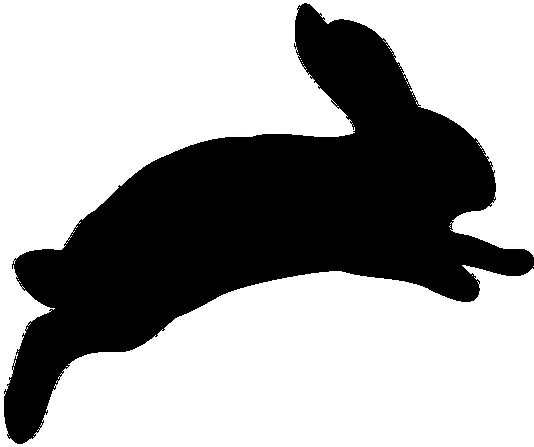
\includegraphics[height = .1\textheight]{rabbit_b}
%       };

%       \node<6->[
%       below = of p_t_false,
%       ] (t_p_t_false) {
%         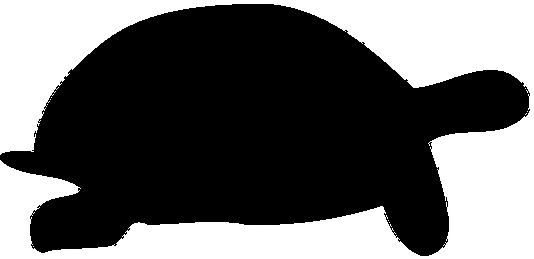
\includegraphics[height = .1\textheight]{turtle_b}
%       };

%       \node<9->[
%       below = of p_f_false,
%       ] (r_p_f_false) {
%         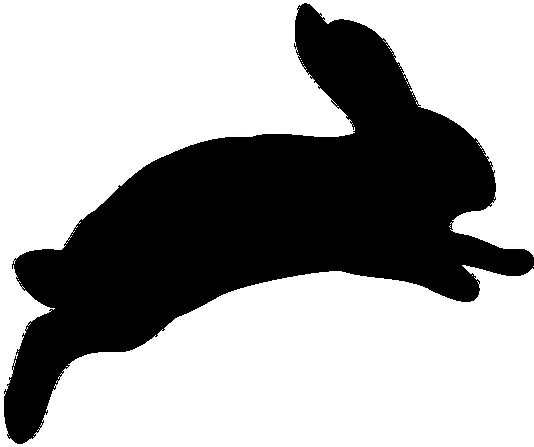
\includegraphics[height = .1\textheight]{rabbit_b}
%       };

%       \node<11->[
%       below = of p_f_true,
%       ] (q_p_f_true) {
%         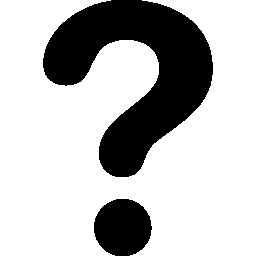
\includegraphics[height = .1\textheight]{question_b}
%       };

%       \draw<2-> (if_bound) -> (true);
%       \draw<3-> (true) -> (p_t_true);
%       \draw<4-> (p_t_true) -> (r_p_t_true);
%       \draw<5-> (true) -> (p_t_false);
%       \draw<6-> (p_t_false) -> (t_p_t_false);
%       \draw<7-> (if_bound) -> (false);
%       \draw<8-> (false) -> (p_f_false);
%       \draw<9-> (p_f_false) -> (r_p_f_false);
%       \draw<10-> (false) -> (p_f_true);
%       \draw<11-> (p_f_true) -> (q_p_f_true);

%     \end{tikzpicture}
%     % \caption{}\label{fig:exe_in_order}
%   \end{figure}

%   \note<1>{

%     Рассмотрим, в каких случаях происходит спекулятивное выполнение.

%   }

%   \note<2>{

%     Если чтение участка памяти происходит согласно заявленным границам.

%   }

%   \note<3>{

%     Чтение согласно границам, предсказатель также думал, что чтение будет
%     происходить согласно границам:

%     \begin{itemize}
%     \item спекулятивно выполнится код чтения в соответствии с границами памяти
%     \end{itemize}

%   }

%   \note<4>{

%     В итоге выполнение кода произойдёт быстро, так как уже заранее был выполнен,
%     результаты получены.

%   }

%   \note<5>{

%     Чтение согласно границам, предсказатель же думал, что чтение памяти выйдет
%     за границы.

%     \begin{itemize}
%     \item спекулятивно будет выполняться последующий за чтением памяти код
%     \item спекулятивное выполнение отбросится, выполнение кода будет происходить
%       заново
%     \end{itemize}

%   }

%   \note<6>{

%     В итоге из-за расхождения реальности с предсказанием, скорость выполнения
%     кода будет ниже.

%   }

%   \note<7>{

%     Если чтение участка памяти происходит за заявленными границами памяти.

%   }

%   \note<8>{

%     Чтение участка памяти за границами, предсказатель также думал, что чтение
%     будет происходить за границами.

%     \begin{itemize}
%     \item спекулятивно будет выполняться последующий за чтением памяти код
%     \end{itemize}

%   }

%   \note<9>{

%     Код исполнится быстро, так как предсказатель угадал и спекулятивно выполнял
%     последующий код.

%   }

%   \note<10>{

%     В случае же, если предсказатель ошибся и решил, что вычисления будут
%     происходить в границах памяти:

%     \begin{itemize}
%     \item спекулятивно выполнится код, который на практике выходит за границы
%       памяти
%     \end{itemize}

%   }

%   \note<11>{

%     \textbf{Спекулятивно выполнится код}, который на практике \textbf{выходит за
%       границы памяти}.

%   }

% \end{frame}

% \subsubsection{Тренировка предсказателя переходов}
% \begin{frame}[fragile]{\insertsubsubsection}

%   \begin{figure}[h]

%     \newcommand*\colorcone{Black}
%     \newcommand*\colorctwo{Black}
%     \newcommand*\colorcthree{Black}
%     \newcommand*\colorcfour{Black}
%     \newcommand*\colorcfive{Black}
%     \newcommand*\colorcsix{Black}
%     \newcommand*\colorcseven{Black}
%     \newcommand*\digitnum{0}

%     \only<2-3> {
%       \renewcommand*\colorcone{BrickRed}
%     }
%     \only<4-5> {
%       \renewcommand*\colorctwo{BrickRed}
%       \renewcommand*\digitnum{1}
%     }
%     \only<6-7> {
%       \renewcommand*\colorcthree{BrickRed}
%       \renewcommand*\digitnum{2}
%     }
%     \only<8-9> {
%       \renewcommand*\colorcfour{BrickRed}
%       \renewcommand*\digitnum{3}
%     }
%     \only<10-11> {
%       \renewcommand*\colorcfive{red}
%       \renewcommand*\digitnum{4}
%     }
%     \only<12-13> {
%       \renewcommand*\colorcsix{red}
%       \renewcommand*\digitnum{5}
%     }
%     \only<14-15> {
%       \renewcommand*\colorcseven{red}
%       \renewcommand*\digitnum{6}
%     }

%     \begin{tikzpicture}[
%       draw,
%       align = center,
%       ->,
%       > = Stealth,
%       thick,
%       double distance = 1pt,
%       node distance = .6,
%       block/.style = {
%         rectangle,
%         draw,
%         fill = ForestGreen,
%         text = White,
%         minimum width = 2cm,
%       },
%       ]

%       \node[
%       ] (code) {
%         \color{Black}index = \color{Mahogany}\digitnum\color{Black};\\
%         \color{Black}char* data = "\color{\colorcone}t\color{\colorctwo}e\color{\colorcthree}x\color{\colorcfour}t\color{\colorcfive}K\color{\colorcsix}E\color{\colorcseven}Y\color{Black}";\\
%         \color{Black}if (index < \color{Mahogany}4\color{Black})\\
%       };

%       \node[
%       below left = 3 of code,
%       text = Black,
%       font = \ttfamily,
%       minimum width = 3cm,
%       ] (cache) {
%         arr1[untrusted]
%       };

%       \node[
%       below = of code,
%       text = White,
%       fill = ForestGreen,
%       draw,
%       label = below:Предсказание,
%       ] (zero) {
%         $\omega = $\\
%         \only<1-2>{.50 | .50}%
%         \only<3-4>{.60 | .40}%
%         \only<5-6>{.69 | .31}%
%         \only<7-8>{.76 | .24}%
%         \only<9-10>{.81 | .19}%
%         \only<11-12>{.77 | .23}%
%         \only<13-14>{.70 | .30}%
%         \only<15>{.64 | .36}%
%       };

%       \node[
%       below right = 3 of code,
%       text = Black,
%       font = \ttfamily,
%       minimum width = 3cm,
%       ] (zero) {
%         0
%       };

%       \draw<1-2,11,13,15> (code) -> node[above, sloped] {true} (cache);
%       \draw<1,3-10,12,14> (code) -> node[above, sloped] {false} (zero);

%       \draw<2>[NavyBlue] (code) -> node[above, sloped] {false} node[below, sloped] {Спекулятивно} (zero);
%       \draw<3>[ForestGreen] (code) -> node[above, sloped] {true} node[below, sloped] {Реально} (cache);

%       \draw<4>[NavyBlue] (code) -> node[above, sloped] {true} node[below, sloped] {Спекулятивно} (cache);
%       \draw<5>[ForestGreen] (code) -> node[above, sloped] {true} node[below, sloped] {Реально} (cache);

%       \draw<6>[NavyBlue] (code) -> node[above, sloped] {true} node[below, sloped] {Спекулятивно} (cache);
%       \draw<7>[ForestGreen] (code) -> node[above, sloped] {true} node[below, sloped] {Реально} (cache);

%       \draw<8>[NavyBlue] (code) -> node[above, sloped] {true} node[below, sloped] {Спекулятивно} (cache);
%       \draw<9>[ForestGreen] (code) -> node[above, sloped] {true} node[below, sloped] {Реально} (cache);

%       \draw<10>[BrickRed] (code) -> node[above, sloped] {true} node[below, sloped] {Спекулятивно} (cache);
%       \draw<11>[ForestGreen] (code) -> node[above, sloped] {false} node[below, sloped] {Реально} (zero);

%       \draw<12>[BrickRed] (code) -> node[above, sloped] {true} node[below, sloped] {Спекулятивно} (cache);
%       \draw<13>[ForestGreen] (code) -> node[above, sloped] {false} node[below, sloped] {Реально} (zero);

%       \draw<14>[BrickRed] (code) -> node[above, sloped] {true} node[below, sloped] {Спекулятивно} (cache);
%       \draw<15>[ForestGreen] (code) -> node[above, sloped] {false} node[below, sloped] {Реально} (zero);

%     \end{tikzpicture}
%     % \caption{Неосознанная тренировка предсказателя переходов}
%   \end{figure}

%   \note<1>{



%   }

% \end{frame}

% \subsubsection{Обход проверки границ}
% \begin{frame}[fragile]{\insertsubsubsection}

%   \begin{minted}{c}
%     struct array {
%       unsigned long length;
%       unsigned char data[];
%     };
%     struct array *arr1 = ...; /* небольшой массив */
%     struct array *arr2 = ...; /* массив размером 0x400 */
%     unsigned long untrusted_offset_from_user = ...;
%     if (untrusted_offset_from_user < arr1->length) {
%       unsigned char value = arr1->data[untrusted_offset_from_user];
%       unsigned long index2 = ((value & 1) * 0x100) + 0x200;
%       if (index2 < arr2->length) {
%         unsigned char value2 = arr2->data[index2];
%       }
%     }
%   \end{minted}

%   \note{

%     Существует множество вариантов эксплуатации данной уязвимости, рассмотрим
%     одну из них.

%     Разберём всё по порядку.

%   }
% \end{frame}

% \begin{frame}[fragile]{\insertsubsubsection}

%   \begin{minted}{c}
%     struct array {
%       unsigned long length;
%       unsigned char data[];
%     };
%     struct array *arr1 = ...; /* небольшой массив */
%     struct array *arr2 = ...; /* массив размером 0x400 */
%   \end{minted}

%   \note{

%     Объявляется два массива.

%     Первый --- целевой массив, в котором будет происходить обход границ.

%     Второй --- массив для применения атаки на кэш.

%   }
% \end{frame}

% \begin{frame}[fragile]{\insertsubsubsection}

%   \begin{minted}{c}
%     /* переменная, управляемая атакующим */
%     unsigned long untrusted_offset_from_user = ...;

%     /* проверка границ */
%     if (untrusted_offset_from_user < arr1->length) {

%       /* спекулятивное выполнение, получение значения недоступной памяти */
%       unsigned char value = arr1->data[untrusted_offset_from_user];

%       /* получение значения бита интересующей области памяти */
%       unsigned long index2 = ((value & 1) * 0x100) + 0x200;

%       /* атака на кэш */
%       unsigned char value2 = arr2->data[index2];
%     }
%   \end{minted}

%   \note{

%     Проверка границ происходит как в примере представленном ранее.

%     Атака на кэш происходит как в примере, рассказанном ранее.

%     Код следующий за проверкой границ называется «гаджетом», как и в случае с
%     ROP.

%     Многое зависит от устройства кэшей различных уровней, TLB, BTB (branch
%     target buffers).

%   }
% \end{frame}

% \subsubsection{ASM}
% \begin{frame}[fragile]{\insertsubsubsection}

%   \begin{minted}{nasm}
%     LDR X1, [X2]      ; X2 - указатель на arr1->length
%     CMP X0, X1        ; X0 содержит untrusted_offset_from_user
%     BGE out_of_range
%     LDRB W4, [X5,X0]  ; X5 содержит arr1->data
%     AND X4, X4, #1
%     LSL X4, X4, #8
%     ADD X4, X4, #0x200
%     LDRB X7, [X8, X4] ; X8 содержит arr2->data
%     out_of_range
%   \end{minted}

%   \note{

%     Упрощённый asm код

%     Спекулятивно можно выполнить так же \textbf{ROP гаджеты}, заставить
%     выполнять операции, тем самым считывать данные из \textbf{закрытых
%       ресурсов}, например, крипто-чип.

%   }

% \end{frame}


\subsubsection{Предотвращение}
\begin{frame}{\insertsubsubsection}

  \begin{itemize}
  \item отключение спекулятивного выполнения
  \item ограничение доступа к высокоточным таймерам
  \item привилегированная очистка кэша
  \item полное изолирование важных данных
  \item вставка инструкций для остановки спекулятивного выполнения
  \end{itemize}

  \note{

    \begin{itemize}
    \item Как отключить? Большое проседание в производительности!
    \item сделали свои таймеры
    \item другие методы очистки
    \item spectre работает и на безопасных анклавах
    \item большое проседание по производительности + всё перекомпилировать
    \end{itemize}

  }

\end{frame}